\documentclass[t]{beamer}
\usecolortheme[RGB={0,114,197}]{structure} 
\usetheme{Ilmenau} 
\usepackage{tikz}
\usepackage{multicol}

\title{Software-Ontwerp}
\subtitle{Iteratie 2}
\author{Reniers V. - Devlieghere J. - Castel D. - Pante S.}
\institute{KU Leuven}

\begin{document}

\frame{\titlepage} 
\begin{frame}{Inhoud}
\begin{multicols}{2}
\tableofcontents
\end{multicols}
\end{frame}



\section{Inleiding} 
\begin{frame}{Inleiding} 
Thema's die aan bod komen:
\begin{itemize}
	\item Ontwerp van MVC.
	\item GRASP en design patterns.
	\item System Sequence Diagram.
	\item Test cases (iteratie 3).
\end{itemize}
\end{frame}

\subsection{Rolverdeling}
\begin{frame}{Rolverdeling}
\begin{multicols}{2}
\tableofcontents[currentsection]
\end{multicols}
\end{frame}

\begin{frame}{Rolverdeling}
Iteratie 2:
\begin{itemize}
	\item Lead Designer: Dieter Castel
	\item Lead Tester: Vincent Reniers
\end{itemize}

Iteratie 3:
\begin{itemize}
	\item Lead Designer: Jonas Devlieghere
	\item Lead Tester: Stefan Pante
	\item Domain Modeler: Vincent Reniers
\end{itemize}
\end{frame}

\subsection{Werkverdeling}

\begin{frame}{Werkverdeling}
Iteratie 2: 1 maart - 15 maart

\begin{center}
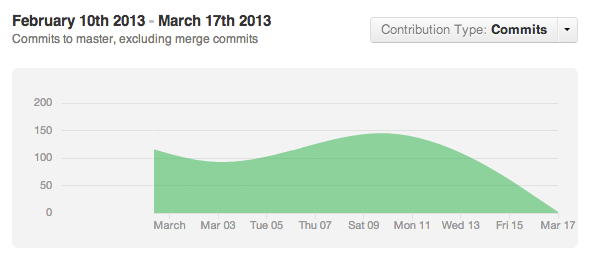
\includegraphics[width= 0.90\linewidth]{images/flowchart}
\end{center}

Uren gepresteerd: 45 uur per persoon.

\end{frame}
\section{Het ontwerp}
\subsection{MVC}

\begin{frame}{MVC}
\begin{center}
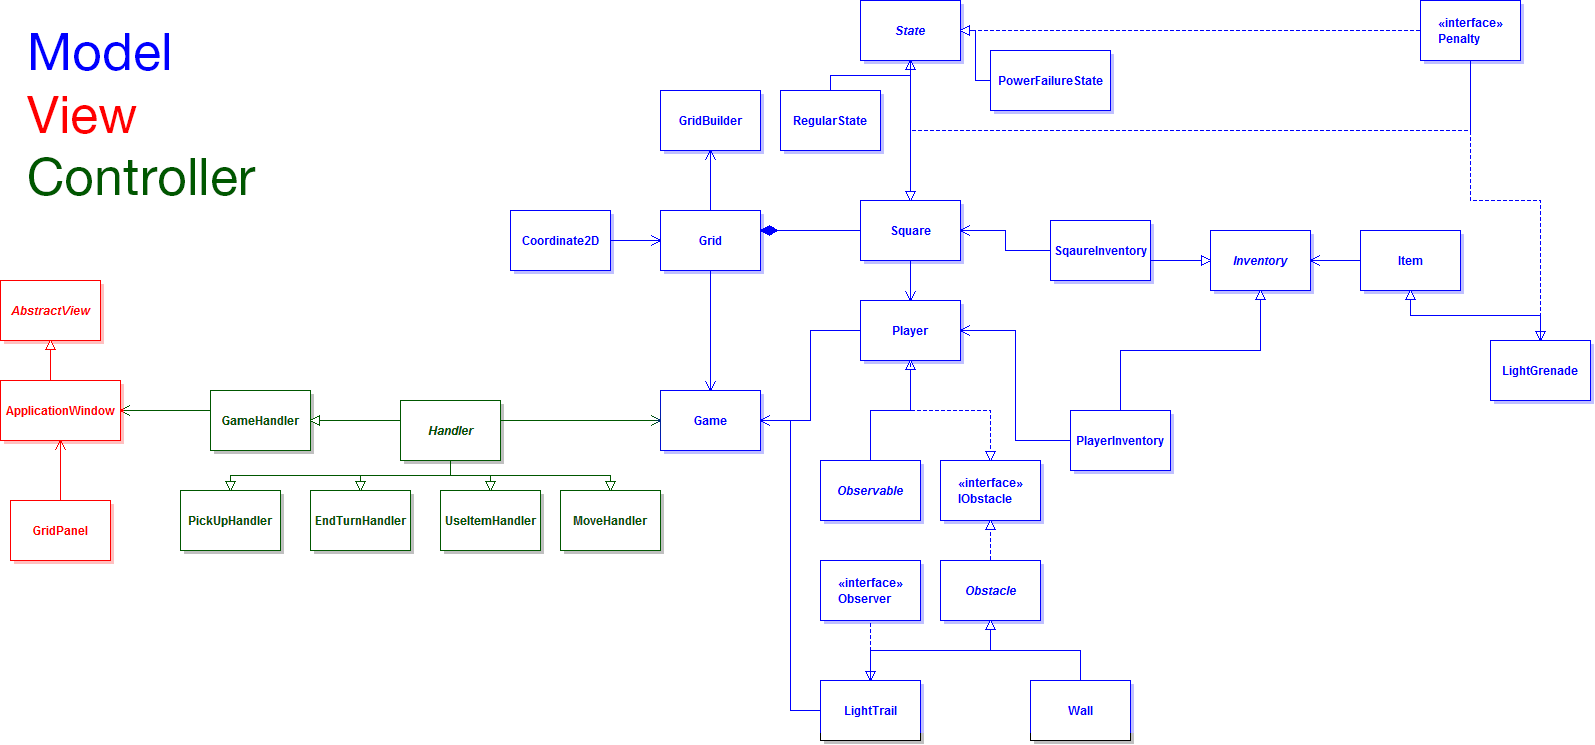
\includegraphics[width=0.90\linewidth]{images/MVC-overview3}
\end{center}
\end{frame}


\begin{frame}{Handlers and view}
\begin{center}
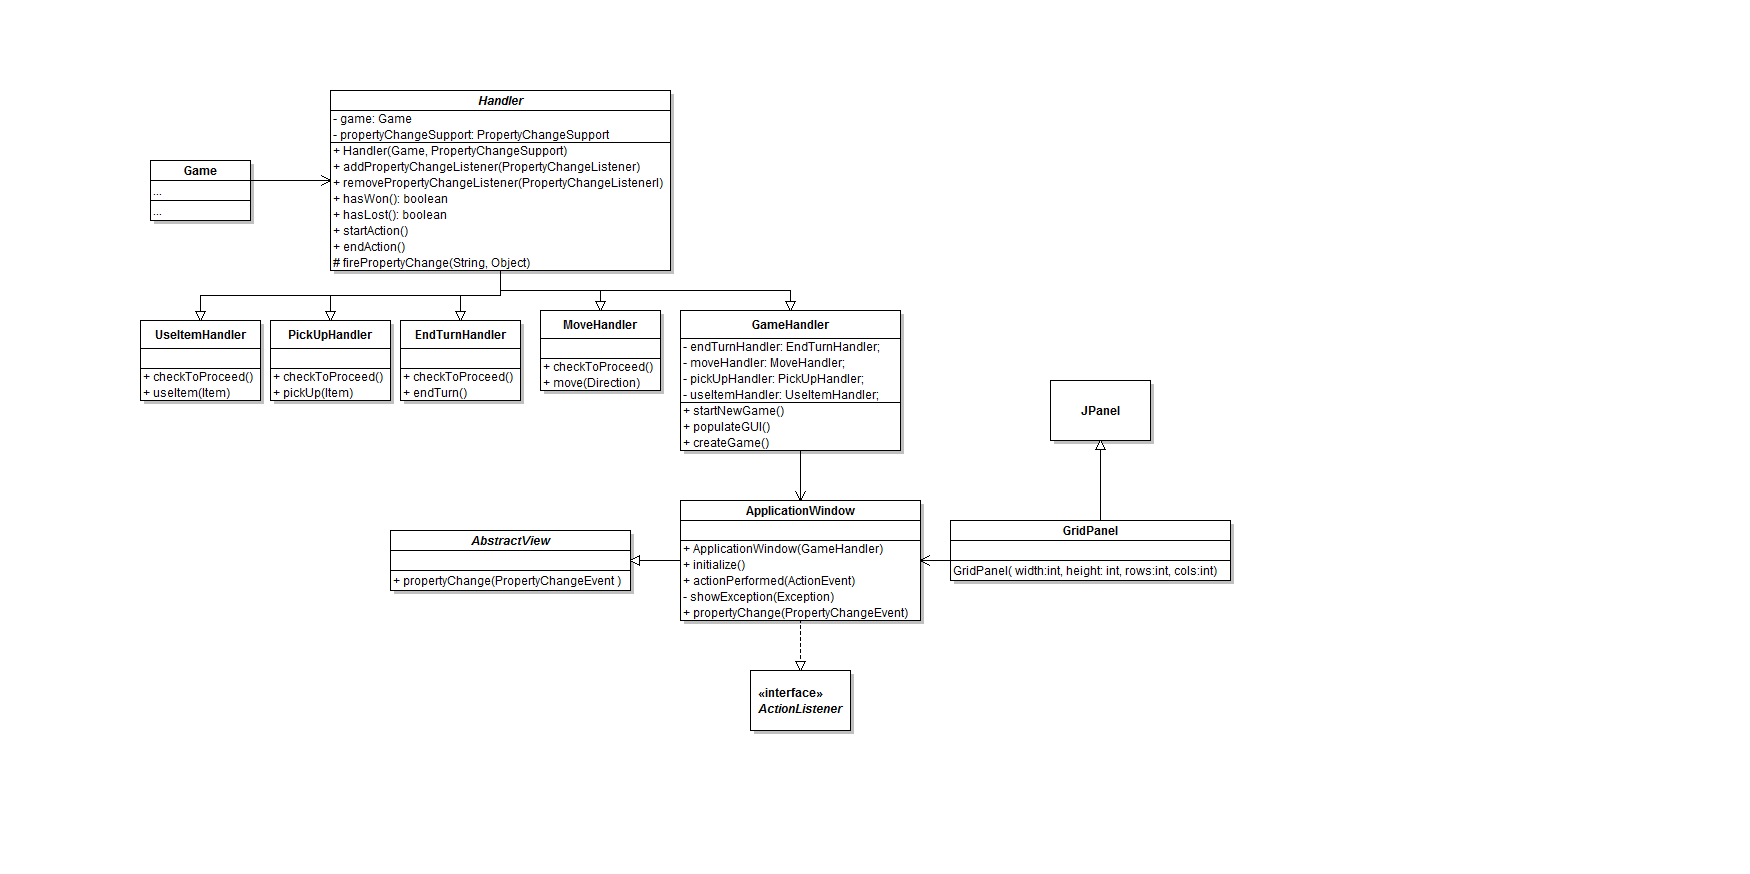
\includegraphics[width=\linewidth]{images/Handlers-View}
\end{center}
\end{frame}


\begin{frame}{Handlers and view}
MVA (Model-View-Adapter) 
\begin{itemize}
	\item Model en View communiceren niet rechtstreeks
	\item Handlers zijn \textbf{mediating controllers}
	\item \textit{ApplicationWindow} implementeert \textit{PropertyChangeListener}
\end{itemize}
Handlers
\begin{itemize}
	\item Handler voor elke Use-Case
	\item Geen GUI controller meer
\end{itemize}
\end{frame}

\subsection{Grid}
\begin{frame}{Grid}
\begin{center}
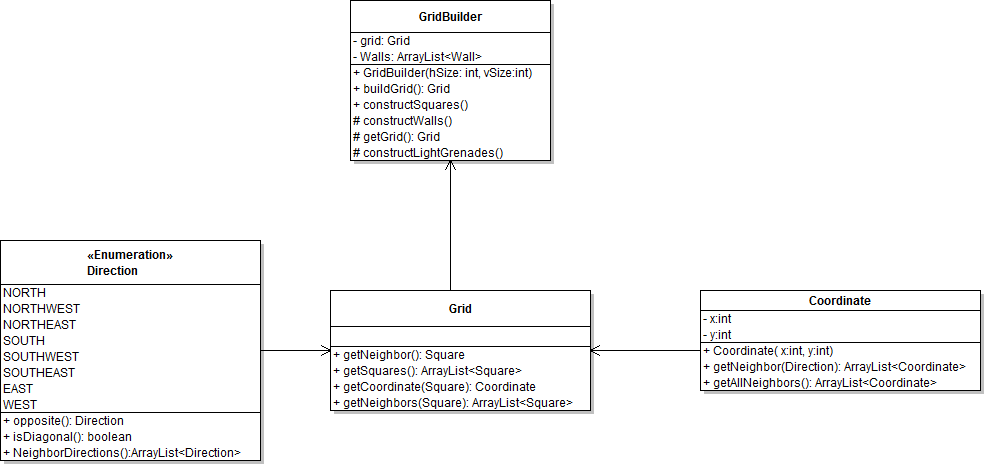
\includegraphics[width=\linewidth]{images/GridClass}
\end{center}
\end{frame}


\subsection{Obstacles}
\begin{frame}{Obstacle}
\begin{center}
\begin{itemize}
	\item Interface \textit{IObstacle}
	\item  Abstracte klasse \textit{Obstacle} implementeert \textit{IObstacle}
	\begin{itemize}
		\item \textit{LightTrail} implementeert \textit{Obstacle}
		\item \textit{Wall} implementeert \textit{Obstacle}
	\end{itemize}
	\item \textit{Player} implementeert \textit{IObstacle}
	\item \textit{Square} kan \textit{Obstacle} bevatten
\end{itemize}
LightTrail implementeert de \textit{Observer} interface.
\end{center}
\end{frame}


\begin{frame}{Obstacle}
\begin{center}
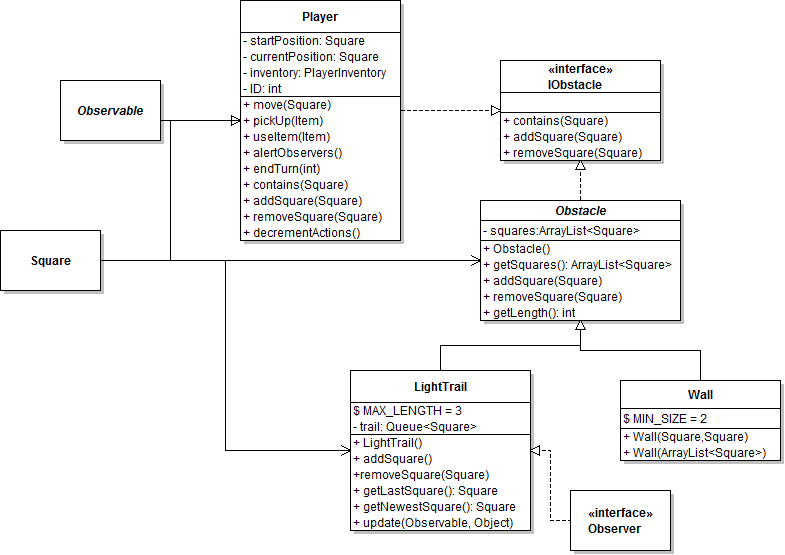
\includegraphics[width=0.70\linewidth]{images/obstacleObserverClassDiagram}
\end{center}
\end{frame}

\subsection{States and Penalty}

\begin{frame}{States and Penalty}
\begin{itemize}
	\item State Pattern
	\begin{itemize}
		\item Square heeft meerdere toestanden: \textit{RegularState}, \textit{PowerFailureState}
		\item Square zorgt voor overgang van staat
	\end{itemize}
	\item Chain of Responsibility (Command)
	\begin{itemize}
		\item State bepaalt eigen penalty
		\item LightGrenade bepaalt eigen penalty
		\item Square is eigenaar van concept penalty
	\end{itemize}
\end{itemize}
\end{frame}

\begin{frame}{States and Penalty}
\begin{center}
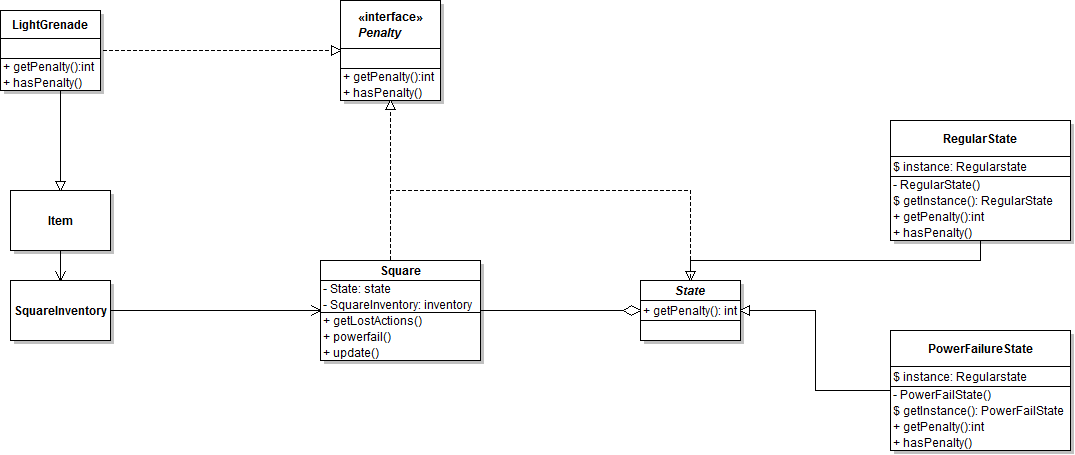
\includegraphics[width=0.90\linewidth]{images/classDiagramStateAndPanelty}
\end{center}
\end{frame}


\section{System State Diagrams}
\subsection{Start New Game}
\begin{frame}{Start New Game}
\begin{center}
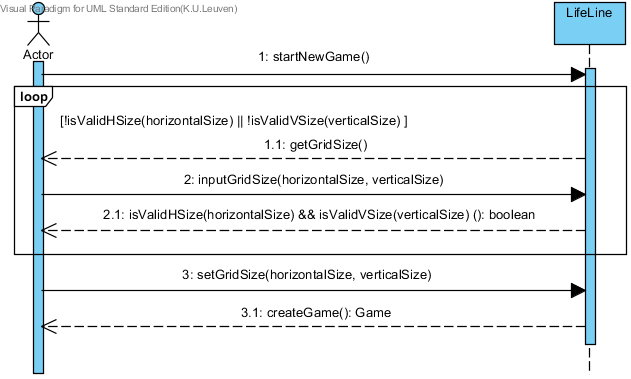
\includegraphics[width=0.90\linewidth]{images/SSDStartNewGame}
\end{center}
\end{frame}

\subsection{Move}
\begin{frame}{Move deel 1}
\begin{center}
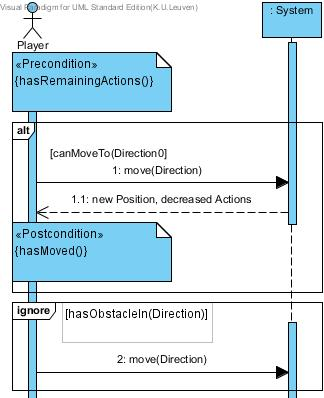
\includegraphics[scale=0.6]{images/SSDMove1}
\end{center}
\end{frame}

\begin{frame}{Move deel 2}
\begin{center}
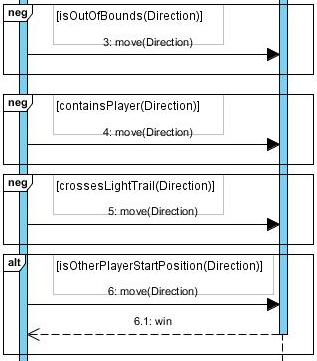
\includegraphics[scale=0.7]{images/SSDMove2}
\end{center}
\end{frame}

\subsection{Pick Up Item}
\begin{frame}{Pick Up Item deel 1}
\begin{center}
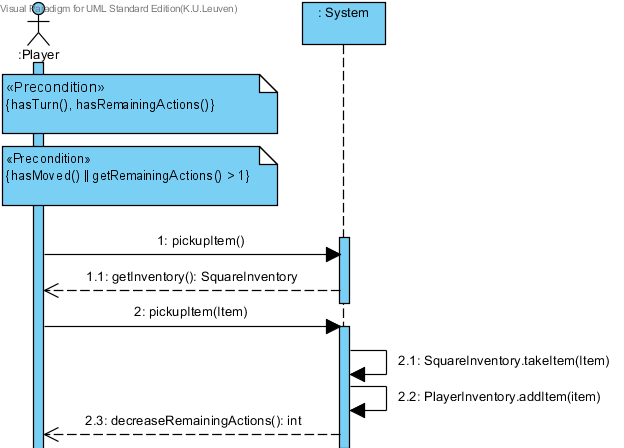
\includegraphics[scale=0.55]{images/SSDPickUpItem1}
\end{center}
\end{frame}

\begin{frame}{Pick Up Item deel 2}
\begin{center}
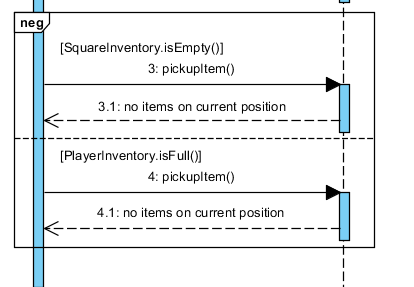
\includegraphics[scale=0.9]{images/SSDPickUpItem2}
\end{center}
\end{frame}


\subsection{Use Item}
\begin{frame}{Use Item deel 1}
\begin{center}
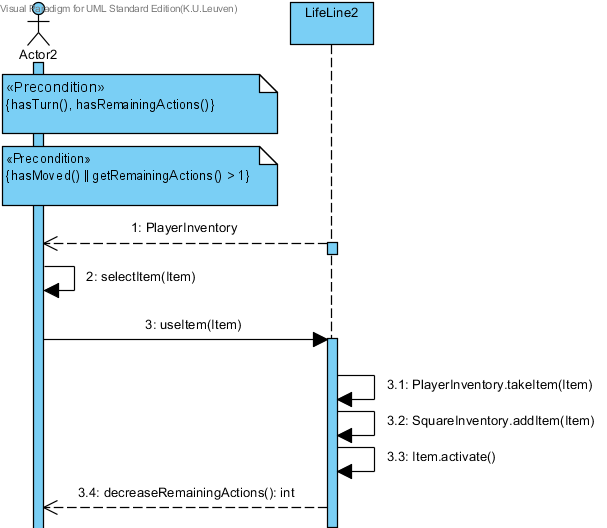
\includegraphics[scale=0.5]{images/SSDUseItem1}
\end{center}
\end{frame}

\begin{frame}{Use Item deel 2}
\begin{center}
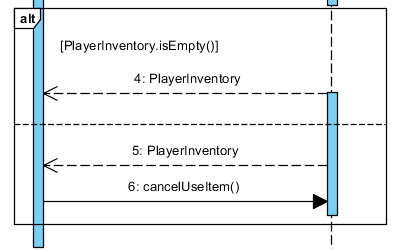
\includegraphics[scale=0.9]{images/SSDUseItem2}
\end{center}
\end{frame}

\subsection{End Turn}
\begin{frame}{End Turn deel 1}
\begin{center}
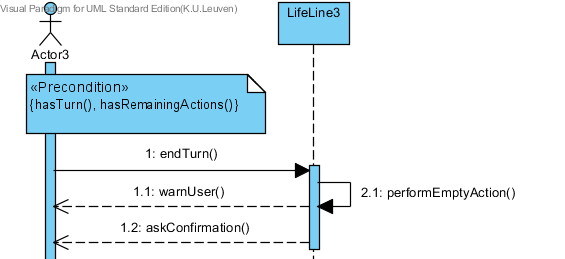
\includegraphics[scale=0.8]{images/SSDEndTurn1}
\end{center}
\end{frame}

\begin{frame}{End Turn deel 2}
\begin{center}
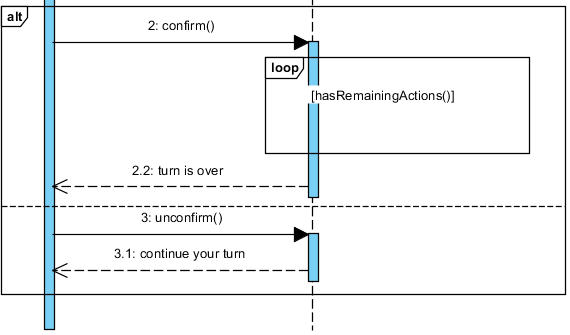
\includegraphics[scale=0.7]{images/SSDEndTurn2}
\end{center}
\end{frame}


\section{Slot}
\begin{frame}{Besluit}
\vspace{0.8in}
\begin{center}
Bedankt voor uw aandacht.
\end{center}
\end{frame}

\end{document}
